\chapter{Plastic Omnium Clean Energy System} \label{Plastic Omnium}
\markboth{\MakeUppercase{Plastic Omnium Clean Energy System}}{\MakeUppercase{Plastic Omnium Clean Energy System}}


The Clean Energy Systems (CES) is one of the three divisions of the Plastic Omnium company, specialised in plastic fuel tanks systems, and depollution systems, mostly for private and commercial vehicles. In 2018, more than 22M fuel systems have been delivered, representing 1 out of 4 commercialised vehicles equipped with a fuel system coming from the CES division.
The material used for producing the fuel tanks is HDPE (High-Density Polyethylene). There are several reasons why they are made of plastic and not in metal as they used to be (for cars):
\begin{itemize}
    \item Plastic is lighter than metal (about 30\%), which allows a reduction of fuel consumption.
    \item The raw material is less expensive.
    \item A plastic tank cannot explode: it will melt, and the fuel will be spilled on the floor.
\end{itemize}

However, one issue is the permeability: as plastic is a porous material, fuel will eventually end up going through it and that leads to two major issues: the consumer will lose some of his gas, and this one will go into the air and pollute the atmosphere. That is why a fuel tank is not a simple container of fuel: it’s a real part composed of complex technologies, from the production processes to the material used, and also the parts attached to the fuel system: filling system, pump gauge module, ventilation. These are used to make the fuel system (Figure \ref{fig:Fuel System}) less permeable to cope with the different regulations.
\begin{figure}
\centerline{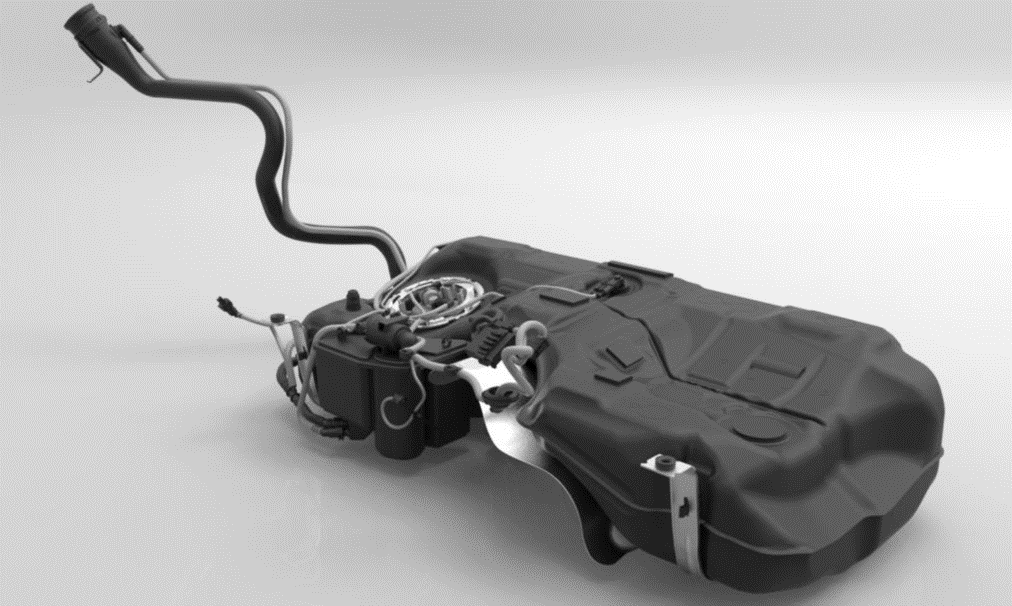
\includegraphics[scale=0.4]{images/appendix_A/fuel_system.png}}
\caption{Fuel System}
\label{fig:Fuel System}
\end{figure}
A fuel system is composed of a fuel tank (Figure \ref{fig:Plastic Fuel Tank}) and a filler pipe (Figure \ref{fig:Filler Pipe}, the latter is the only part visible of the system by the end user, to refill the tank at the station.

\begin{figure}
\centerline{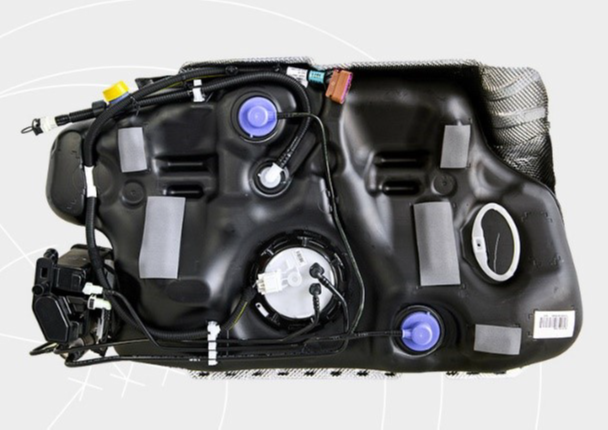
\includegraphics[scale=0.6]{images/appendix_A/Plastic_fuel_tank.png}}
\caption{Plastic Fuel Tank}
\label{fig:Plastic Fuel Tank}
\end{figure}
\begin{figure}
\centerline{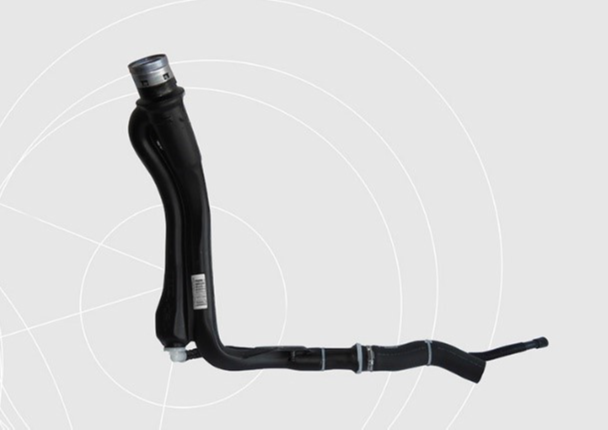
\includegraphics[scale=0.6]{images/appendix_A/Filler_pipe.png}}
\caption{Filler Pipe}
\label{fig:Filler Pipe}
\end{figure}

The SCR technology (Selective Catalytic Reduction) is an effective response to the regulatory requirements limiting emissions of nitrogen oxides ($NO_x$) from diesel vehicles. Combining a tank with a pump and gauge module, this system injects vaporised \textit{AdBlue®} into the hot exhaust gases, causing a chemical reaction that transforms $NO_x$ into water vapor. Plastic Omnium CES has developed a range of SCR systems to meet the needs of all types of vehicles, from the smallest European city car to the largest American pickup truck.